% Options for packages loaded elsewhere
\PassOptionsToPackage{unicode}{hyperref}
\PassOptionsToPackage{hyphens}{url}
%
\documentclass[
]{book}
\usepackage{amsmath,amssymb}
\usepackage{iftex}
\ifPDFTeX
  \usepackage[T1]{fontenc}
  \usepackage[utf8]{inputenc}
  \usepackage{textcomp} % provide euro and other symbols
\else % if luatex or xetex
  \usepackage{unicode-math} % this also loads fontspec
  \defaultfontfeatures{Scale=MatchLowercase}
  \defaultfontfeatures[\rmfamily]{Ligatures=TeX,Scale=1}
\fi
\usepackage{lmodern}
\ifPDFTeX\else
  % xetex/luatex font selection
\fi
% Use upquote if available, for straight quotes in verbatim environments
\IfFileExists{upquote.sty}{\usepackage{upquote}}{}
\IfFileExists{microtype.sty}{% use microtype if available
  \usepackage[]{microtype}
  \UseMicrotypeSet[protrusion]{basicmath} % disable protrusion for tt fonts
}{}
\makeatletter
\@ifundefined{KOMAClassName}{% if non-KOMA class
  \IfFileExists{parskip.sty}{%
    \usepackage{parskip}
  }{% else
    \setlength{\parindent}{0pt}
    \setlength{\parskip}{6pt plus 2pt minus 1pt}}
}{% if KOMA class
  \KOMAoptions{parskip=half}}
\makeatother
\usepackage{xcolor}
\usepackage{color}
\usepackage{fancyvrb}
\newcommand{\VerbBar}{|}
\newcommand{\VERB}{\Verb[commandchars=\\\{\}]}
\DefineVerbatimEnvironment{Highlighting}{Verbatim}{commandchars=\\\{\}}
% Add ',fontsize=\small' for more characters per line
\usepackage{framed}
\definecolor{shadecolor}{RGB}{248,248,248}
\newenvironment{Shaded}{\begin{snugshade}}{\end{snugshade}}
\newcommand{\AlertTok}[1]{\textcolor[rgb]{0.94,0.16,0.16}{#1}}
\newcommand{\AnnotationTok}[1]{\textcolor[rgb]{0.56,0.35,0.01}{\textbf{\textit{#1}}}}
\newcommand{\AttributeTok}[1]{\textcolor[rgb]{0.13,0.29,0.53}{#1}}
\newcommand{\BaseNTok}[1]{\textcolor[rgb]{0.00,0.00,0.81}{#1}}
\newcommand{\BuiltInTok}[1]{#1}
\newcommand{\CharTok}[1]{\textcolor[rgb]{0.31,0.60,0.02}{#1}}
\newcommand{\CommentTok}[1]{\textcolor[rgb]{0.56,0.35,0.01}{\textit{#1}}}
\newcommand{\CommentVarTok}[1]{\textcolor[rgb]{0.56,0.35,0.01}{\textbf{\textit{#1}}}}
\newcommand{\ConstantTok}[1]{\textcolor[rgb]{0.56,0.35,0.01}{#1}}
\newcommand{\ControlFlowTok}[1]{\textcolor[rgb]{0.13,0.29,0.53}{\textbf{#1}}}
\newcommand{\DataTypeTok}[1]{\textcolor[rgb]{0.13,0.29,0.53}{#1}}
\newcommand{\DecValTok}[1]{\textcolor[rgb]{0.00,0.00,0.81}{#1}}
\newcommand{\DocumentationTok}[1]{\textcolor[rgb]{0.56,0.35,0.01}{\textbf{\textit{#1}}}}
\newcommand{\ErrorTok}[1]{\textcolor[rgb]{0.64,0.00,0.00}{\textbf{#1}}}
\newcommand{\ExtensionTok}[1]{#1}
\newcommand{\FloatTok}[1]{\textcolor[rgb]{0.00,0.00,0.81}{#1}}
\newcommand{\FunctionTok}[1]{\textcolor[rgb]{0.13,0.29,0.53}{\textbf{#1}}}
\newcommand{\ImportTok}[1]{#1}
\newcommand{\InformationTok}[1]{\textcolor[rgb]{0.56,0.35,0.01}{\textbf{\textit{#1}}}}
\newcommand{\KeywordTok}[1]{\textcolor[rgb]{0.13,0.29,0.53}{\textbf{#1}}}
\newcommand{\NormalTok}[1]{#1}
\newcommand{\OperatorTok}[1]{\textcolor[rgb]{0.81,0.36,0.00}{\textbf{#1}}}
\newcommand{\OtherTok}[1]{\textcolor[rgb]{0.56,0.35,0.01}{#1}}
\newcommand{\PreprocessorTok}[1]{\textcolor[rgb]{0.56,0.35,0.01}{\textit{#1}}}
\newcommand{\RegionMarkerTok}[1]{#1}
\newcommand{\SpecialCharTok}[1]{\textcolor[rgb]{0.81,0.36,0.00}{\textbf{#1}}}
\newcommand{\SpecialStringTok}[1]{\textcolor[rgb]{0.31,0.60,0.02}{#1}}
\newcommand{\StringTok}[1]{\textcolor[rgb]{0.31,0.60,0.02}{#1}}
\newcommand{\VariableTok}[1]{\textcolor[rgb]{0.00,0.00,0.00}{#1}}
\newcommand{\VerbatimStringTok}[1]{\textcolor[rgb]{0.31,0.60,0.02}{#1}}
\newcommand{\WarningTok}[1]{\textcolor[rgb]{0.56,0.35,0.01}{\textbf{\textit{#1}}}}
\usepackage{longtable,booktabs,array}
\usepackage{calc} % for calculating minipage widths
% Correct order of tables after \paragraph or \subparagraph
\usepackage{etoolbox}
\makeatletter
\patchcmd\longtable{\par}{\if@noskipsec\mbox{}\fi\par}{}{}
\makeatother
% Allow footnotes in longtable head/foot
\IfFileExists{footnotehyper.sty}{\usepackage{footnotehyper}}{\usepackage{footnote}}
\makesavenoteenv{longtable}
\usepackage{graphicx}
\makeatletter
\def\maxwidth{\ifdim\Gin@nat@width>\linewidth\linewidth\else\Gin@nat@width\fi}
\def\maxheight{\ifdim\Gin@nat@height>\textheight\textheight\else\Gin@nat@height\fi}
\makeatother
% Scale images if necessary, so that they will not overflow the page
% margins by default, and it is still possible to overwrite the defaults
% using explicit options in \includegraphics[width, height, ...]{}
\setkeys{Gin}{width=\maxwidth,height=\maxheight,keepaspectratio}
% Set default figure placement to htbp
\makeatletter
\def\fps@figure{htbp}
\makeatother
\setlength{\emergencystretch}{3em} % prevent overfull lines
\providecommand{\tightlist}{%
  \setlength{\itemsep}{0pt}\setlength{\parskip}{0pt}}
\setcounter{secnumdepth}{5}
\usepackage{booktabs}
\ifLuaTeX
  \usepackage{selnolig}  % disable illegal ligatures
\fi
\usepackage[]{natbib}
\bibliographystyle{plainnat}
\usepackage{bookmark}
\IfFileExists{xurl.sty}{\usepackage{xurl}}{} % add URL line breaks if available
\urlstyle{same}
\hypersetup{
  pdftitle={Aprendizagem de Máquina},
  pdfauthor={Giseldo Neo},
  hidelinks,
  pdfcreator={LaTeX via pandoc}}

\title{Aprendizagem de Máquina}
\author{Giseldo Neo}
\date{}

\begin{document}
\maketitle

{
\setcounter{tocdepth}{1}
\tableofcontents
}
\begin{verbatim}
## -- Attaching core tidyverse packages ------------------------ tidyverse 2.0.0 --
## v dplyr     1.1.4     v readr     2.1.5
## v forcats   1.0.0     v stringr   1.5.1
## v ggplot2   3.5.0     v tibble    3.2.1
## v lubridate 1.9.3     v tidyr     1.3.1
## v purrr     1.0.2     
## -- Conflicts ------------------------------------------ tidyverse_conflicts() --
## x dplyr::filter() masks stats::filter()
## x dplyr::lag()    masks stats::lag()
## i Use the conflicted package (<http://conflicted.r-lib.org/>) to force all conflicts to become errors
\end{verbatim}

\chapter*{Prefácil}\label{prefuxe1cil}
\addcontentsline{toc}{chapter}{Prefácil}

Este livro visa dar ao leitor uma visão prática e teórica sobre aprendizagem de máquina e estatística com exemplos de programação em R e em Python.

\section*{Sobre}\label{sobre}
\addcontentsline{toc}{section}{Sobre}

Todos os direitos reservados, proibida a redistribuição

\section*{O autor}\label{o-autor}
\addcontentsline{toc}{section}{O autor}

Giseldo Neo é Mestre em Modelagem Computacional e Professor.

\chapter{Introdução}\label{introduuxe7uxe3o}

Thomas H. Davenport e DJ Patil publicaram uma matéria de opinião em 2012 na conceituada revista de administração e negócios Harvard Business Review afirmando que um dos empregos mais sexy do século 21 seria o cientista de dados (termo cunhado pelo próprio DJ Patil) e deu um exemplo do crescimento em visualizações do linkedin quando foi utilizado o recurso de pessoas que talvez você conheça, recurso este que utilizava a extensa base de dados de conexões do linkedin para fazer um cruzamento do tipo: se uma pessoa qualquer conhece fulano e fulano conhece ciclano então essa pessoa qualquer tem grande chance de conhecer ciclano \citep{hbr2012}. Porém, acredito que outras pessoas possam ter visões diferentes do que é um emprego sexy, como por exemplo Joel Grus (2016) \citep{grus2016}.

Particularmente, a escolha do que é ser sexy foge do escopo desse livro. Porém, existe um relativo consenso de que o campo está em evidência. Muitas pesquisas estão sendo escritas sobre esse tema, com experimentos e achados importantes. Logo, a habilidade em lidar com esses dados e reportá-los é crucial para o profissional que deseja extrair informação útil e construir conhecimento.

Vamos começar pelos conceitos básicos e criar um vocabulário consistente nas seções seguintes.

\chapter{Classificação do dado}\label{classificauxe7uxe3o-do-dado}

Vamos classificar o dado em categorias que nos permitirão uma comunicação mais consistente e com menos redundância. Essas classificações facilitarão a nossa comunicação.

\section{Dado e informação}\label{dado-e-informauxe7uxe3o}

Dado e informação são coisas diferentes. Os dados são os fatos brutos. Por exemplo, o nome de um estudante e o número do CPF são exemplos de dados brutos.

Informação é quando utilizamos os dados aplicados em um contexto. Por exemplo, os dados do nome e do CPF de um estudante podem fazer parte de uma lista de alunos matriculados em um curso técnico de informática de um Instituto Federal. Os dados organizados agora trazem uma informação associada.

Apesar dessa divisão teórica entre dado e informação, os termos serão usados indiscriminadamente aqui e com o mesmo significado. Também chamaremos no texto dado como variável, ou atributo

\section{Tipo do dado (Qualitativo ou Quantitativo)}\label{tipo-do-dado-qualitativo-ou-quantitativo}

É necessário classificar o dado quanto ao seu tipo pois os algoritmos de aprendizagem de máquina, ou os modelos estatísticos de inferência (termos que serão explicados mais a frente), irão funcionar com determinados tipos de determinadas formas. Logo, com o conhecimento da classificação do tipo do dado poderemos realizar, ou não, as conversões ou tratamentos adicionais que forem necessários.

Utilizaremos dois tipos de dados principais o \textbf{qualitativo} e \textbf{quantitativo}.

O tipo do dado pode ser: \textbf{quantitativo} (também chamado de numérico); \textbf{qualitativo} (também chamado de categórico); ou se enquadram na categoria \textbf{especial} que engloba outros tipos.

Um dado do tipo \textbf{quantitativo} é expresso geralmente como um número. Porém, existem casos em que números inteiros também expressam dados do tipo \textbf{qualitativo,} portanto não é só ter número que já podemos classificá-lo como \textbf{quantitativo}.

Já o dado do tipo \textbf{qualitativo} está relacionado a um valor dentro de um conjunto de itens geralmente finito, porém nem sempre.

Por exemplo, a formação acadêmica de uma determinada pessoa, que pode ser Ensino Fundamental completo, Médio completo ou Superior completo, é um dado do tipo \textbf{qualitativo}. Já o salário de um trabalhador é um dado to tipo \textbf{quantitativo}.

\subsection{Quantitativo}\label{quantitativo}

O tipo do dado \textbf{quantitativo}, também chamado de numérico, ainda pode ser sub classificado como \textbf{quantitativo contínuo} ou \textbf{quantitativo discreto}.

Um dado \textbf{quantitativo contínuo} é quando o dado pode ser qualquer número em um intervalo de números reais - lembrando que o conjunto de número reais engloba os números inteiros -. Geralmente é o resultado de uma medida, por exemplo, a altura de um estudante (por exemplo 1,80 metros) é um dado do tipo \textbf{quantitativo contínuo}.

O dado \textbf{quantitativo discreto} geralmente é resultado de uma contagem - um número inteiro -, por exemplo, a idade de um estudante (42 anos) é uma contagem, é um dado \textbf{quantitativo discreto}.

\subsection{Qualitativo}\label{qualitativo}

Um dado é do tipo \textbf{qualitativo} quando representa um valor dentro de um conjunto ou de uma categoria.

O dado \textbf{qualitativo} pode ser \textbf{qualitativo} \textbf{binário} ou \textbf{qualitativo} \textbf{ordinal}, ou nenhuma das duas subcategorias, ou seja \textbf{qualitativo} \textbf{somente}.

Um exemplo de \textbf{dado qualitativo} \textbf{somente}, é a cor preferida por uma pessoa (por exemplo eu prefiro a cor azul), ou o estado civil de uma pessoa.

O dado do tipo \textbf{qualitativo} \textbf{binário} é quando ele somente pode assumir dois valores no universo de valores possíveis. Por exemplo, 0 ou 1, existente ou ausente, true ou false, sim e não, aprovado ou reprovado.

O dado do tipo \textbf{qualitativo} \textbf{ordinal} é quando o valor é um elemento de um conjunto que pode ser ordenado, por exemplo, imagine a classificação dos seres humanos entre criança, jovem e adulto. Nesse exemplo, existe uma ordem temporal, o jovem já foi uma criança, o adulto já foi um jovem.

\subsection{Exemplos}\label{exemplos}

\begin{longtable}[]{@{}
  >{\raggedright\arraybackslash}p{(\columnwidth - 2\tabcolsep) * \real{0.4722}}
  >{\raggedright\arraybackslash}p{(\columnwidth - 2\tabcolsep) * \real{0.5278}}@{}}
\toprule\noalign{}
\begin{minipage}[b]{\linewidth}\raggedright
Variável
\end{minipage} & \begin{minipage}[b]{\linewidth}\raggedright
Tipo do dado
\end{minipage} \\
\midrule\noalign{}
\endhead
\bottomrule\noalign{}
\endlastfoot
Idade (14, 17, 23) & \textbf{quantitativo} discreto \\
Doença (Ausente, Presente) & \textbf{qualitativo} binário \\
Story Points (1, 3, 5, 7 \ldots{} ) & \textbf{qualitativo} ordinal \\
Ano (2021, 2022, \ldots) & \textbf{quantitativo} discreto \\
Altura (1,79 - 2,05 - \ldots) & \textbf{quantitativo} contínuo \\
Estado Civil (Casado, Solteiro) & \textbf{qualitativo} binário \\
Cores preferidas (Azul, verde, vermelho) & \textbf{qualitativo} \textbf{somente} (nem binário, nem ordinal) \\
\end{longtable}

\section{Tipo do dado (Preditor, Alvo)}\label{tipo-do-dado-preditor-alvo}

Nos modelos de aprendizagem de máquina (quando lidamos com algoritmos classificados como supervisionados) e de inferência estatistica o dado também pode ser classificado entre atributo preditor ou atributo alvo. Atributo preditor, são os atributos que serão utilizados para realizar a previsão, geralmente um ou mais atributos. Atributo alvo é o atributo que queremos `advinhar (ou dar o melhor chute técnico)' com os modelos preditivos. Atributo preditor muitas vezes é chamado de vairável independente, e atributo alvo de variável dependente.

\begin{longtable}[]{@{}
  >{\raggedright\arraybackslash}p{(\columnwidth - 4\tabcolsep) * \real{0.2500}}
  >{\raggedright\arraybackslash}p{(\columnwidth - 4\tabcolsep) * \real{0.3750}}
  >{\raggedright\arraybackslash}p{(\columnwidth - 4\tabcolsep) * \real{0.3750}}@{}}
\toprule\noalign{}
\begin{minipage}[b]{\linewidth}\raggedright
Col1
\end{minipage} & \begin{minipage}[b]{\linewidth}\raggedright
Tipo do dado (numerico ou categorico)
\end{minipage} & \begin{minipage}[b]{\linewidth}\raggedright
Tipo do atributo (preditor ou alvo)
\end{minipage} \\
\midrule\noalign{}
\endhead
\bottomrule\noalign{}
\endlastfoot
IssueKey & categorigo somente & - \\
StoryPoint & numerico discreto & alvo \\
Created & data & - \\
Title & texto & preditor \\
Desription & texto & preditor \\
\end{longtable}

Ou seja, no modelo proposto, o título e a descrição serão os atributos preditores do atributo alvo, espera-se que os dados do título e da descrição contenham as informações necessárias para a estimativa em Story Points.

\section{Tabelas}\label{tabelas}

Os dados geralmente são organizados em formato de tabelas. Onde as linhas representam as obseravações (ou instâncias) e as colunas representam as variáveis.

Vamos utilizar o exemplo de uma empresa que desenvolve software e registra os dados relacionados a seus projetos. Essa empresa mantem o registro de determinada funcionalidade e do tamanho dessa funcionalidade. Cada linha da tabela representa uma funcionalidade (chamada de User Story em projetos que utilizam SCRUM). Cada coluna representa uma informação dessa User Story. As informações que a empresa mantém registro são as variáveis, as colunas da tabela. Uma dessas variáveis é a descriçao, outra é uma estimativa que o desenvolvedor atribui do tamanho funional, chamado Story Point. Essas informações estão dispostas em um arquivo no formato CSV. O código abaixo, carrega esse arquivo e exibe parte de seu conteúdo. Iremos então classificar cada uma das colunas de acordo com o tipo do dado.

Código R

\begin{Shaded}
\begin{Highlighting}[]
\NormalTok{df }\OtherTok{\textless{}{-}} \FunctionTok{read\_csv}\NormalTok{(}\StringTok{\textquotesingle{}data/neodataset/7764.csv\textquotesingle{}}\NormalTok{)}
\end{Highlighting}
\end{Shaded}

\begin{verbatim}
## Rows: 355 Columns: 5
## -- Column specification --------------------------------------------------------
## Delimiter: ","
## chr  (2): title, description
## dbl  (2): issuekey, storypoints
## dttm (1): created
## 
## i Use `spec()` to retrieve the full column specification for this data.
## i Specify the column types or set `show_col_types = FALSE` to quiet this message.
\end{verbatim}

\begin{Shaded}
\begin{Highlighting}[]
\FunctionTok{head}\NormalTok{(df)}
\end{Highlighting}
\end{Shaded}

\begin{verbatim}
## # A tibble: 6 x 5
##   issuekey created             title                     description storypoints
##      <dbl> <dttm>              <chr>                     <chr>             <dbl>
## 1 29688087 2020-01-17 00:50:48 Update templates for web~ "Relates t~           1
## 2 29682716 2020-01-16 19:21:38 Make sure that we Captur~ "This was ~           1
## 3 29644971 2020-01-15 21:17:03 Propose new IA for Brand~ "## Goals\~           1
## 4 29494181 2020-01-10 19:20:50 Cache `node_modules` for~ "# UPDATE ~           1
## 5 29437529 2020-01-09 10:26:51 Disable all remaining un~ "Similar t~           1
## 6 29358963 2020-01-07 08:35:44 Disable unnecessary jobs~ "As discus~           1
\end{verbatim}

Código Python

\begin{Shaded}
\begin{Highlighting}[]
\ImportTok{import}\NormalTok{ pandas }\ImportTok{as}\NormalTok{ pd}
\CommentTok{\#pd.set\_option(\textquotesingle{}max\_columns\textquotesingle{}, None)}
\NormalTok{df }\OperatorTok{=}\NormalTok{ pd.read\_csv(}\StringTok{\textquotesingle{}data/neodataset/7764.csv\textquotesingle{}}\NormalTok{)}
\NormalTok{df.head()}
\end{Highlighting}
\end{Shaded}

\begin{verbatim}
##    issuekey  ... storypoints
## 0  29688087  ...           1
## 1  29682716  ...           1
## 2  29644971  ...           1
## 3  29494181  ...           1
## 4  29437529  ...           1
## 
## [5 rows x 5 columns]
\end{verbatim}

A tabela abaixo não é um exemplo dos dados é a classificação, note que o que era antes coluna virou linha.

\begin{longtable}[]{@{}
  >{\raggedright\arraybackslash}p{(\columnwidth - 4\tabcolsep) * \real{0.2500}}
  >{\raggedright\arraybackslash}p{(\columnwidth - 4\tabcolsep) * \real{0.2500}}
  >{\raggedright\arraybackslash}p{(\columnwidth - 4\tabcolsep) * \real{0.5000}}@{}}
\toprule\noalign{}
\begin{minipage}[b]{\linewidth}\raggedright
Nome da Coluna
\end{minipage} & \begin{minipage}[b]{\linewidth}\raggedright
Tipo do dado
\end{minipage} & \begin{minipage}[b]{\linewidth}\raggedright
Observação
\end{minipage} \\
\midrule\noalign{}
\endhead
\bottomrule\noalign{}
\endlastfoot
Issuekey & categorico somente & Apesar de ser um número, não são realizadas operações no número, ele é um identificador único da User Story \\
storypoints & numérico discreto & É um número geralmente de 1 á 100 \\
created & data & Data em que a User Story Foi criada \\
title & texto & Título da User Story \\
description & texto & Desrição da User Story \\
\end{longtable}

A tabela acima apresenta a caracterização dos dados do conjunto de dados neodataset (esse conjunto de dados pode ser baixado em \ldots). Nessa tabela foram tipificados os dados. É interessante apresentar essa tipificação em estudos cientificos e trabalhos de conclusão de curso, quando estamos lidando com conjuntos de dados. Cabe ressaltar que essa tipificação independe da linguagem. Internamente cada linguagem de programação tem seus tipos especificos e que podem ter pequenas diferenças entre as linguagens.

\chapter{Estimativas de localização}\label{estimativas-de-localizauxe7uxe3o}

Muitas vezes é conveniente representar um conjunto de números de uma forma mais simples. Nem sempre temos a possibilidade de lidar com vários números, por limitação ou por falta de praticidade. Por exemplo, imagine uma sala de aula com 5 estudantes, vamos montar uma lista da idade de todos os estudantes nessa sala no R e no Python, duas linguagens de programação comumente utilizadas em análise de dados.

O código a seguir criar uma lista com 5 idades e depois imprime essa mesma lista na linguagem R

\begin{Shaded}
\begin{Highlighting}[]
\NormalTok{idades }\OtherTok{\textless{}{-}} \FunctionTok{c}\NormalTok{(}\DecValTok{14}\NormalTok{,}\DecValTok{15}\NormalTok{,}\DecValTok{16}\NormalTok{,}\DecValTok{14}\NormalTok{,}\DecValTok{17}\NormalTok{)}
\NormalTok{idades}
\end{Highlighting}
\end{Shaded}

\begin{verbatim}
## [1] 14 15 16 14 17
\end{verbatim}

O código a seguir criar uma lista com 5 idades e depois imprime essa mesma lista na linguagem Python

\begin{Shaded}
\begin{Highlighting}[]
\NormalTok{idades }\OperatorTok{=}\NormalTok{ [}\DecValTok{14}\NormalTok{, }\DecValTok{15}\NormalTok{, }\DecValTok{16}\NormalTok{, }\DecValTok{14}\NormalTok{, }\DecValTok{17}\NormalTok{] }
\BuiltInTok{print}\NormalTok{(idades)}
\end{Highlighting}
\end{Shaded}

\begin{verbatim}
## [14, 15, 16, 14, 17]
\end{verbatim}

Podemos representar essa lista com um número mais simples, que pode resumir ou representar aquela lista original. Para isso, utilizamos as estimativas de localização \citep{bruce2020practical}. As mais comuns são média e mediana.

\section{Média}\label{muxe9dia}

A média é calculada dividindo a soma de todos os números da lista pela quantidade de itens. Sua fórmula matemática é apresentada em FIGURA XXX. Onde i é a quantidade de itens da lista e \(x_i\) é o enésimo item da lista. O termo média também pode ser representado pelo símbolo \(X\)

No nosso exemplo se fossemos calcular manualmente a média da lista idade, o cálculo seria:

Código R

\{r\} ( 14 + 15 + 16 + 14 + 17 ) / 5

Código Python

\{python\} print(( 14 + 15 + 16 + 14 + 17 ) / 5)

Porém, podemos utilizar algumas funções que já disponibilizam esse recurso de calular a média. O código para criar uma lista e verificar a média dessa lista, utilizando as funções, no R e no Python, seria o seguinte:

Código R

\{r\} idades \textless- c(14, 15, 16, 14, 17) mean(idades)

Código Python

\{python\} from statistics import mean idades = {[}14, 15, 16, 14, 17{]} print(mean(idades))

A função mean, no R, recebe como parâmetro uma lista de itens e retorna a média dessa lista, no python utilizei a função mesmo nome, porém disponível na biblioteca statistics do python.

\chapter{Análise exploratória dos dados}\label{anuxe1lise-exploratuxf3ria-dos-dados}

\section{Introdução}\label{introduuxe7uxe3o-1}

Um dos pioneiros na definição da área de análise exploratória de dados (em inglês Estatistical Data Analisys, ou EDA) foi Tukey (1997) \citep{tukey1977exploratory}. Tukey (1997) argumenta que seu foco, até aquele momento, estava em desenvolver novas técnicas para inferência. Porém, depois de reflexão, ele chega a conclusão de que o foco dele, e de outros estatísticos, seria melhor aplicado no desenvolvimento de técnicas para a etapa de preparação desses dados. Era nos procedimentos de estruturar os dados que estava o verdadeiro desafio. Problemas, tais como, lidar com dados faltantes ou \emph{outliers,} traziam impactos negativos na inferência e novas técnicas nessa etapa precisavam ser estudadas. Sua recomendação era uma mudança de paradigma e novos estudos, voltando mais para a preparação dos dados. Sua visão é de que isso iria trazer enorme avanços como um todo. O que de fato aconteceu.

Podemos considerar essa necessidade de estudos anterior ao processo de inferência analisando o exemplo criado por Ancobe.

R

\begin{verbatim}
## 
## Attaching package: 'data.table'
\end{verbatim}

\begin{verbatim}
## The following objects are masked from 'package:lubridate':
## 
##     hour, isoweek, mday, minute, month, quarter, second, wday, week,
##     yday, year
\end{verbatim}

\begin{verbatim}
## The following objects are masked from 'package:dplyr':
## 
##     between, first, last
\end{verbatim}

\begin{verbatim}
## The following object is masked from 'package:purrr':
## 
##     transpose
\end{verbatim}

\begin{Shaded}
\begin{Highlighting}[]
\NormalTok{x }\OtherTok{\textless{}{-}} \FunctionTok{c}\NormalTok{(}\DecValTok{10}\NormalTok{, }\DecValTok{8}\NormalTok{, }\DecValTok{13}\NormalTok{, }\DecValTok{9}\NormalTok{, }\DecValTok{11}\NormalTok{, }\DecValTok{14}\NormalTok{, }\DecValTok{6}\NormalTok{, }\DecValTok{4}\NormalTok{ , }\DecValTok{12}\NormalTok{, }\DecValTok{7}\NormalTok{, }\DecValTok{5}\NormalTok{)}
\NormalTok{y }\OtherTok{\textless{}{-}} \FunctionTok{c}\NormalTok{(}\FloatTok{8.04}\NormalTok{, }\FloatTok{6.95}\NormalTok{, }\FloatTok{7.58}\NormalTok{, }\FloatTok{8.81}\NormalTok{, }\FloatTok{8.33}\NormalTok{, }\FloatTok{9.96}\NormalTok{, }\FloatTok{7.24}\NormalTok{, }\FloatTok{4.26}\NormalTok{, }\FloatTok{10.84}\NormalTok{, }\FloatTok{4.82}\NormalTok{, }\FloatTok{5.68}\NormalTok{)}
\NormalTok{DT }\OtherTok{=} \FunctionTok{data.table}\NormalTok{(x, y)}
\FunctionTok{ggplot}\NormalTok{(DT, }\AttributeTok{mapping =} \FunctionTok{aes}\NormalTok{(}\AttributeTok{x =}\NormalTok{ x, }\AttributeTok{y =}\NormalTok{y)) }\SpecialCharTok{+}
  \FunctionTok{geom\_point}\NormalTok{() }\SpecialCharTok{+}
  \FunctionTok{labs}\NormalTok{(}\AttributeTok{title =} \StringTok{"Amostra 1"}\NormalTok{)}
\end{Highlighting}
\end{Shaded}

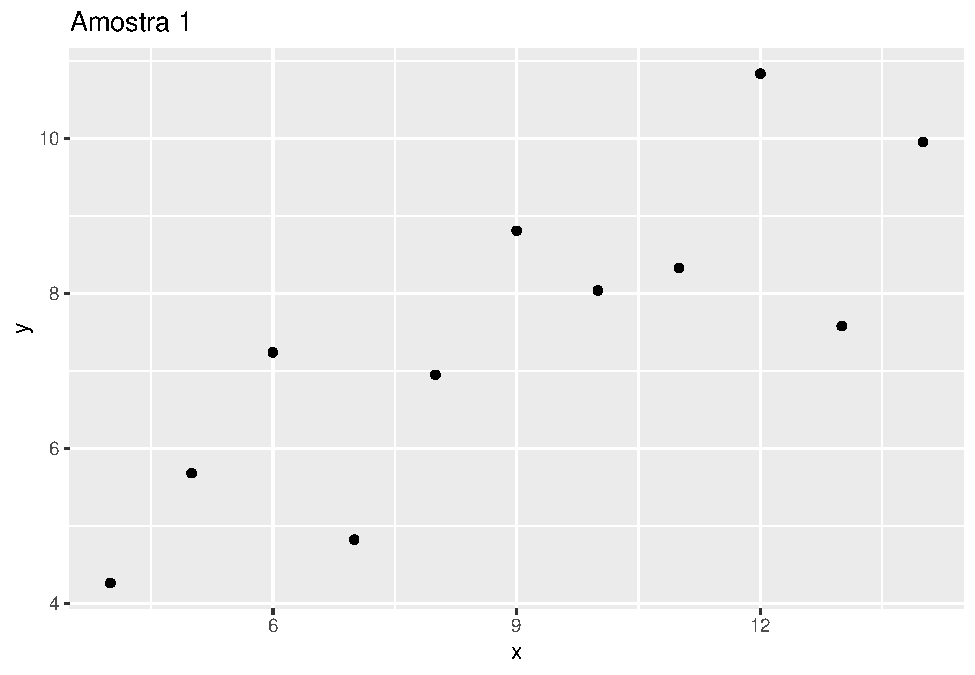
\includegraphics{_main_files/figure-latex/unnamed-chunk-7-1.pdf}

Python

\begin{Shaded}
\begin{Highlighting}[]
\ImportTok{import}\NormalTok{ matplotlib.pyplot }\ImportTok{as}\NormalTok{ plt}
\NormalTok{x }\OperatorTok{=}\NormalTok{ [}\DecValTok{10}\NormalTok{, }\DecValTok{8}\NormalTok{, }\DecValTok{13}\NormalTok{, }\DecValTok{9}\NormalTok{, }\DecValTok{11}\NormalTok{, }\DecValTok{14}\NormalTok{, }\DecValTok{6}\NormalTok{, }\DecValTok{4}\NormalTok{ , }\DecValTok{12}\NormalTok{, }\DecValTok{7}\NormalTok{, }\DecValTok{5}\NormalTok{]}
\NormalTok{y }\OperatorTok{=}\NormalTok{ [}\FloatTok{8.04}\NormalTok{, }\FloatTok{6.95}\NormalTok{, }\FloatTok{7.58}\NormalTok{, }\FloatTok{8.81}\NormalTok{, }\FloatTok{8.33}\NormalTok{, }\FloatTok{9.96}\NormalTok{, }\FloatTok{7.24}\NormalTok{, }\FloatTok{4.26}\NormalTok{, }\FloatTok{10.84}\NormalTok{, }\FloatTok{4.82}\NormalTok{, }\FloatTok{5.68}\NormalTok{]}
\NormalTok{plt.scatter(x, y)}
\NormalTok{plt.show()}
\end{Highlighting}
\end{Shaded}

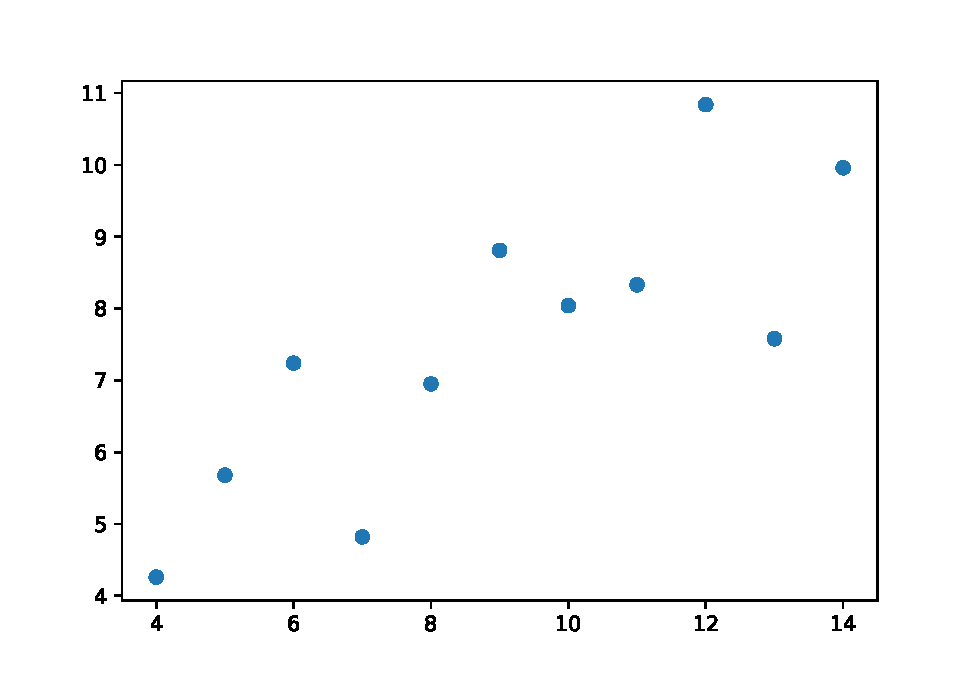
\includegraphics{_main_files/figure-latex/unnamed-chunk-8-1.pdf}

Veja a imagem ``Amostra 1'' acima. Nela visualmente percebemos uma relação linear direta entre as duas variáveis, podemos confirmar isso analisando o gráfico de pontos e o valor da correlação, abaixo.

R

\begin{Shaded}
\begin{Highlighting}[]
\FunctionTok{cor}\NormalTok{(x, y)  }
\end{Highlighting}
\end{Shaded}

\begin{verbatim}
## [1] 0.8164205
\end{verbatim}

Python

\begin{Shaded}
\begin{Highlighting}[]
\ImportTok{from}\NormalTok{ statistics }\ImportTok{import}\NormalTok{ correlation}
\BuiltInTok{print}\NormalTok{(correlation(x, y))}
\end{Highlighting}
\end{Shaded}

\begin{verbatim}
## 0.81642051634484
\end{verbatim}

Para os dados da Amostra 1, acima temos uma correlação de 0.81.

R

\begin{Shaded}
\begin{Highlighting}[]
\NormalTok{x }\OtherTok{\textless{}{-}} \FunctionTok{c}\NormalTok{(}\DecValTok{10}\NormalTok{, }\DecValTok{8}\NormalTok{, }\DecValTok{13}\NormalTok{, }\DecValTok{9}\NormalTok{, }\DecValTok{11}\NormalTok{, }\DecValTok{14}\NormalTok{, }\DecValTok{6}\NormalTok{, }\DecValTok{4}\NormalTok{ , }\DecValTok{12}\NormalTok{, }\DecValTok{7}\NormalTok{, }\DecValTok{5}\NormalTok{)}
\NormalTok{y }\OtherTok{\textless{}{-}} \FunctionTok{c}\NormalTok{(}\FloatTok{9.14}\NormalTok{, }\FloatTok{8.14}\NormalTok{, }\FloatTok{8.74}\NormalTok{,}\FloatTok{8.77}\NormalTok{,}\FloatTok{9.26}\NormalTok{,}\FloatTok{8.1}\NormalTok{,}\FloatTok{6.13}\NormalTok{,}\FloatTok{3.1}\NormalTok{,}\FloatTok{9.11}\NormalTok{,}\FloatTok{7.26}\NormalTok{,}\FloatTok{4.74}\NormalTok{)}
\NormalTok{DT }\OtherTok{=} \FunctionTok{data.table}\NormalTok{(x, y)}
\FunctionTok{ggplot}\NormalTok{(DT, }\AttributeTok{mapping =} \FunctionTok{aes}\NormalTok{(}\AttributeTok{x =}\NormalTok{ x, }\AttributeTok{y =}\NormalTok{y)) }\SpecialCharTok{+}
  \FunctionTok{geom\_point}\NormalTok{() }\SpecialCharTok{+}
  \FunctionTok{labs}\NormalTok{(}\AttributeTok{title =} \StringTok{"Amostra 2"}\NormalTok{)}
\end{Highlighting}
\end{Shaded}

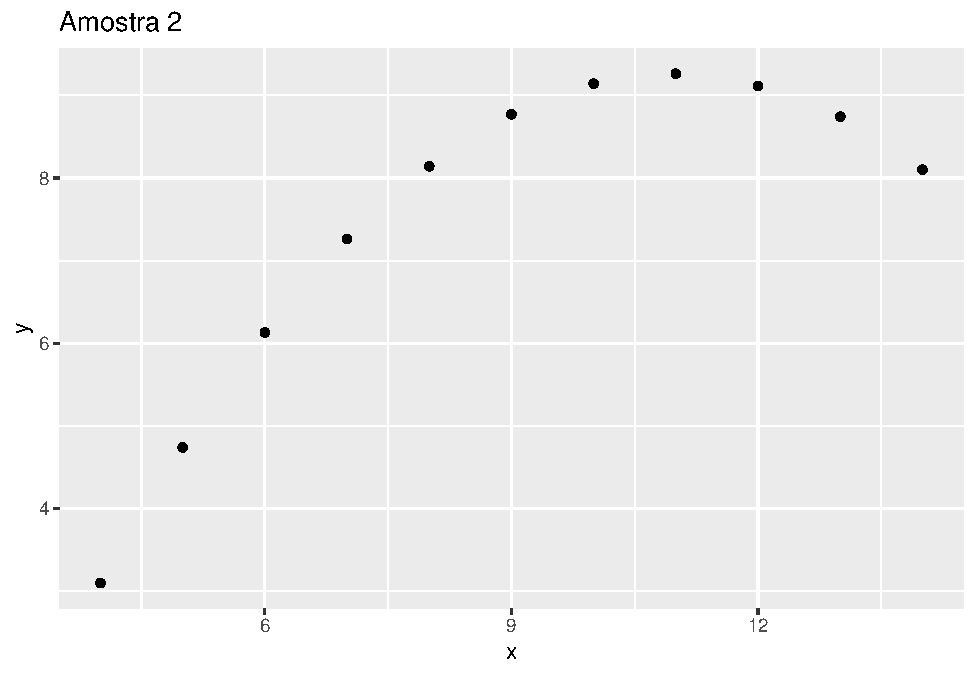
\includegraphics{_main_files/figure-latex/unnamed-chunk-11-1.pdf}

Python

\begin{Shaded}
\begin{Highlighting}[]
\ImportTok{import}\NormalTok{ matplotlib.pyplot }\ImportTok{as}\NormalTok{ plt}
\NormalTok{plt.plot([}\DecValTok{0}\NormalTok{, }\DecValTok{1}\NormalTok{, }\DecValTok{2}\NormalTok{, }\DecValTok{3}\NormalTok{])}
\NormalTok{plt.show()}
\end{Highlighting}
\end{Shaded}

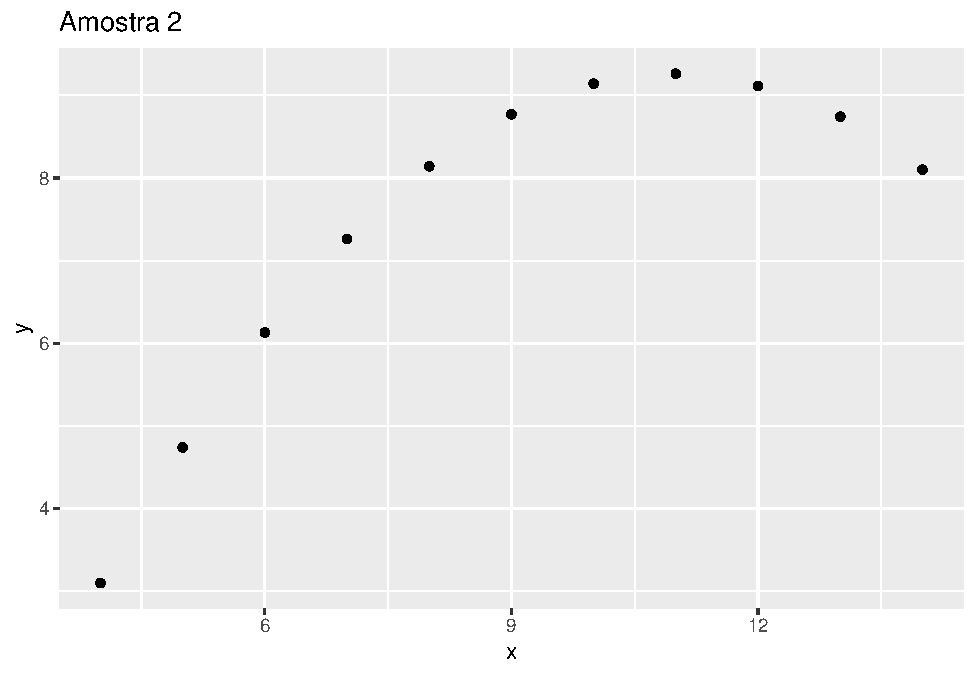
\includegraphics{_main_files/figure-latex/unnamed-chunk-12-1.pdf}

Na amostra 2 percebemos uma relação em forma de curva, quando verificamos a correlação verificamos o mesmo valor de 0.81 dos dados da amostra 1.

\chapter{Python}\label{python}

Com python é possível realizar operações matemáticas, tais como, soma, divisão ou multiplicação, direto no interpretador de codigo.

\begin{Shaded}
\begin{Highlighting}[]
\BuiltInTok{print}\NormalTok{(}\DecValTok{2}\OperatorTok{+}\DecValTok{2}\NormalTok{)}
\end{Highlighting}
\end{Shaded}

\begin{verbatim}
## 4
\end{verbatim}

\chapter{Referências}\label{referuxeancias}

  \bibliography{book.bib,packages.bib}

\end{document}
